\section{Introduction}\label{sec:intro}

Let $X$ be a smooth complex projective variety. A class in $H^{2p}(X,\QQ)$ is
a \emph{Hodge class} if its image in $H^{2p}(X,\CC)$ lies in $H^{p,p}(X)$, and
it is \emph{algebraic} if it is a rational linear combination of the classes
of subvarieties of codimension~$p$. Algebraic classes are Hodge classes. Hodge
asked for the converse \cite{Hod52}.

\begin{conjecture}[Hodge]\label{conj:hodge}
For every smooth complex projective variety $X$ and every $p\ge0$, every
Hodge class in $H^{2p}(X,\QQ)$ is algebraic.
\end{conjecture}

We write \HC{} for this statement. It holds for $p\le1$ and $p\ge\dim X-1$, so
for every variety of dimension at most three, and it is open in general. The
question in the title has a precise form: \emph{from which of the statements
that the literature has isolated does \HC{} follow?} This paper answers that
question, proves the conditional theorems that the answer allows, and stops
at the first statement on each route that we cannot prove. We do not prove
the Hodge conjecture, and no statement below should be read as a claim that
it holds.\footnote{Here and below a statement is called \emph{proved} when
it is proved in this paper or in refereed work. Results that are available
only as preprints are marked as such where they are used. The one preprint
on which a theorem of this paper depends, \cite{OAI26}, enters only as an
explicit hypothesis.}

\subsection*{The statements}
The following statements are made precise in \Cref{def:statements}.
\begin{itemize}[leftmargin=2.6em]
\item[\st{F2}] The Hodge conjecture for abelian varieties.
\item[\st{F3$'$}] The Hodge conjecture modulo abelian varieties: every Hodge
class on every $X$ is a sum of classes $\Gamma_{*}\gamma$, where $\gamma$ is
a Hodge class on an abelian variety $B$ and $\Gamma$ is an algebraic cycle on
$B\times X$.
\item[\st{L}] The Lefschetz standard conjecture $B(X)$ of Grothendieck
\cite{Gro69}, for every $X$.
\item[\st{M}] Every Hodge class is motivated in the sense of Andr\'e
\cite{And96}.
\item[\st{V}] The variational Hodge conjecture: in a smooth projective
family over a smooth connected base, a flat family of rational classes that
is algebraic on one fibre is algebraic on every fibre.
\item[\st{CM}] The Hodge conjecture for abelian varieties of CM type.
\item[\st{IP}] Propagation from CM points: \st{V} for polarized abelian
schemes and classes that are algebraic on a fibre of CM type.
\end{itemize}
The statement \st{CM} is the main theorem claimed in the preprint
\cite{OAI26}, which has not been refereed. We have not verified its proof,
and \Cref{ssec:cmclaim} says which parts of it we have checked.

\begin{maintheorem}\label{thm:A}
The following are equivalent:
\begin{enumerate}[label=\textup{(\roman*)}]
\item \HC;
\item \st{F2} and \st{F3$'$};
\item \st{L} and \st{F3$'$};
\item \st{V} and \st{F3$'$};
\item \st{CM}, \st{IP} and \st{F3$'$};
\item \st{L} and \st{M}.
\end{enumerate}
\end{maintheorem}

The implications from (ii)--(vi) to (i) combine known theorems of Andr\'e,
Deligne, Abdulali and Milne with two observations of this paper:
\st{F3$'$} implies \st{M} (\Cref{prop:f3m}), and \st{CM} together with
\st{IP} implies \st{F2} (\Cref{prop:cmip}). The theorem is proved in
\Cref{ssec:proofA}. The next theorem says that these are all the ways in
which the conjecture follows from the statements above, together with the
other statements the paper meets: the semiregularity of Schoen's subvariety
(\Cref{q:schoen}), and the Hodge conjecture for Fermat varieties and for the
Weil classes of the split Weil families over $\QQ(\sqrt{-3})$.

\begin{maintheorem}[The routes]\label{thm:B}
Let $S$ be a set of the statements of \Cref{tab:rules} that does not contain
\HC, and suppose that \HC{} follows from $S$ by the implications of
\Cref{tab:rules}. Then
\begin{enumerate}[label=\textup{(\alph*)}]
\item either $S$ contains \st{F3$'$} together with one of \st{F2}, \st{L},
\st{V}, or both of \st{CM} and \st{IP};
\item or $S$ contains both \st{L} and \st{M}.
\end{enumerate}
Each of the five minimal sets so described implies \HC, and each implies
every statement of \Cref{tab:rules} except the semiregularity of Schoen's
subvariety.
\end{maintheorem}

So there are two ways in. One passes through abelian varieties and needs
\st{F3$'$} together with a statement that implies \st{F2}; the other avoids
abelian varieties and assumes \st{L} and \st{M}, which by \Cref{thm:A} is the
Hodge conjecture in another form. In particular \st{F2} and \st{F3$'$} can be
avoided as hypotheses, but never as consequences, and Schoen's subvariety
lies on no route at all (\Cref{cor:bypass}). The routes are drawn in
\Cref{fig:routes}.

\begin{figure}[t]
\centering
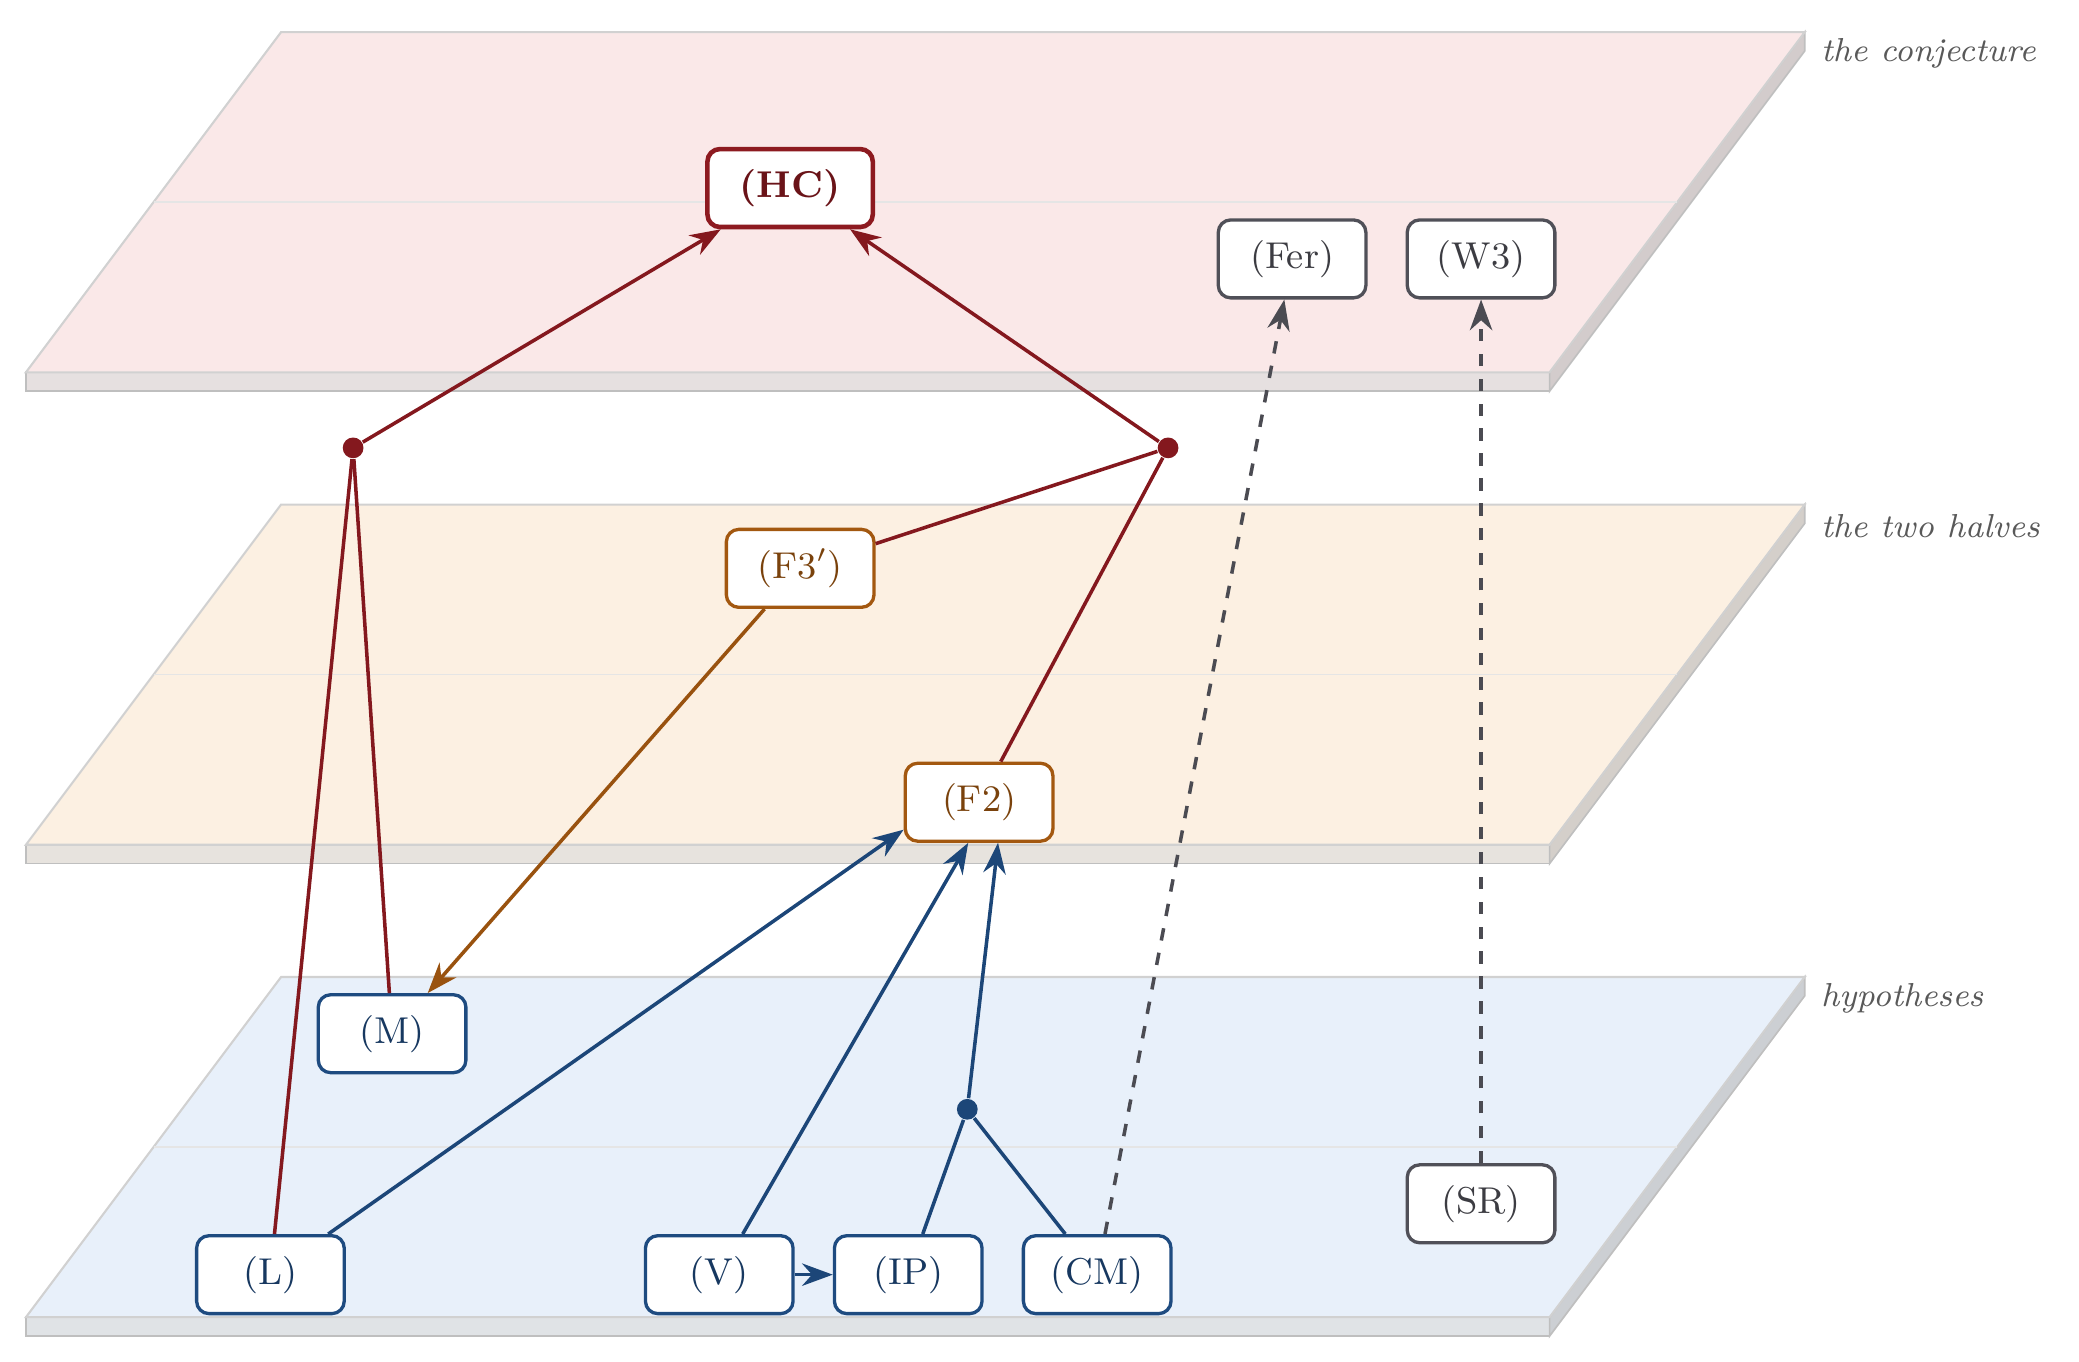
\includegraphics[width=\textwidth]{figures/fig_routes}
\caption{The routes of \Cref{thm:B}. Hypotheses lie on the bottom layer,
the two halves \st{F2} and \st{F3$'$} in the middle, and \HC{} on top.
Arrows are implications of \Cref{tab:rules}. At each dot two lines combine
into a conjunction: $\st{CM}\wedge\st{IP}\Rightarrow\st{F2}$,
$\st{L}\wedge\st{M}\Rightarrow\HC$ and $\st{F2}\wedge\st{F3$'$}\Rightarrow
\HC$. The arrows from \HC{} and \st{F2} to the statements they contain are
not drawn. The dashed arrows on the right lead to the special cases
\st{Fer} and \st{W3} of \Cref{sec:routes}, and not to \HC.}
\label{fig:routes}
\end{figure}

The remaining results are conditional on one statement, or prove one case.
Let $X^{n}_{m}\subseteq\PP^{n+1}$ be the Fermat variety
$x_{0}^{m}+\dots+x_{n+1}^{m}=0$.

\begin{maintheorem}\label{thm:C}
Assume \st{CM}. Then the Hodge conjecture holds for every Fermat variety
$X^{n}_{m}$, for every product of Fermat varieties of any degrees and
dimensions, and for every smooth projective variety onto which such a
product maps surjectively. Without any hypothesis, \st{F3$'$} holds for all
of these varieties.
\end{maintheorem}

Fermat varieties are the first varieties on which the conjecture was
studied in every dimension \cite{Ran80,Shi79}, and unconditional proofs are
known only for special degrees (\Cref{rem:fermatknown}); \Cref{thm:F} below
adds the fourfolds of odd degree. The proof of
\Cref{thm:C} uses the inductive structure of Shioda and Katsura \cite{SK79}
to dominate every Fermat variety by a product of Fermat curves, blown up
along smooth centres, and the fact that Fermat curves have Jacobians of CM
type.

Abelian varieties of Weil type are where \st{F2} is hardest. On the split
Weil family of an imaginary quadratic field over its Shimura variety $S$
(\Cref{ssec:weilfamilies}), write $\Sigma\subseteq S$ for the set of members
on which the Weil classes are algebraic, and $\Sigma_{d}\subseteq\Sigma$ for
the set where they have algebraic representatives of degree at most $d$
(\Cref{def:sigmad}).

\begin{maintheorem}\label{thm:D}
Each $\Sigma_{d}$ is Zariski closed in $S$, and $\Sigma=\bigcup_{d}\Sigma_{d}$.
The following are equivalent:
\begin{enumerate}[label=\textup{(\roman*)}]
\item $\Sigma=S$;
\item $\Sigma_{d}=S$ for some $d$;
\item for some $d$, the CM points in $\Sigma_{d}$ are not contained in any
finite union of proper special subvarieties of $S$.
\end{enumerate}
Under \st{CM} every CM point of $S$ lies in $\Sigma$.
\end{maintheorem}

So under \st{CM} the Weil classes are algebraic on the whole family exactly
when, at the CM points, they have algebraic representatives of uniformly
bounded degree on a set that is not trapped in finitely many proper Shimura
subvarieties. The equivalence of (ii) and (iii) is where the
Andr\'e--Oort conjecture, proved by Pila, Shankar and Tsimerman
\cite{PST21}, enters.

The last result concerns the only cycles known to represent Weil classes at
members with maximal Hodge group in every dimension, those constructed by
Schoen \cite{Sch88}. Let $X$ be a curve of genus $n+1\ge3$, let $C\to X$ be
the \'etale cyclic triple cover given by a line bundle of order three, and
let $B$ be its Prym variety, an abelian variety of dimension $2n$ of Weil
type for $\QQ(\sqrt{-3})$ with polarization class $\eta$.

\begin{maintheorem}\label{thm:E}
There is an irreducible subvariety $Y\subseteq B$ of dimension $n$, built
from one of the three components into which Schoen's cover splits over the
canonical system of $X$, whose class pairs nontrivially with the Weil
classes of $B$. If the Hodge group of $B$ is maximal, which holds for very
general $(X,C)$, then
\[
  \cl(Y)=c\,\eta^{n}+w,\qquad c\in\QQ_{>0},\quad 0\ne w\ \text{a Weil class}.
\]
If $Y$ is semiregular for one such $B$, the Weil classes are algebraic on
every member of the split Weil family of $\QQ(\sqrt{-3})$ in dimension $2n$.
\end{maintheorem}

For $n\le3$ this family is already covered by Schoen's work \cite{Sch88,Sch98}.
For $n\ge4$ it is not: the Prym locus has
dimension $3n$ and the family has dimension $n^{2}$, so $Y$ would have to
deform in $n^{2}-3n$ further directions. The proof of the pairing in \Cref{thm:E} is a short computation with
twisted coefficients on the symmetric product of $X$, and it also gives a
proof of Schoen's theorem that $B$ carries algebraic Weil classes
(\Cref{cor:schoen}). We give the evidence on both sides of \Cref{q:schoen}
in \Cref{ssec:whereitstops}, including a precise analogy
with the Abel--Jacobi curve, which is not semiregular, and with a question
of Markman about a weak form of the semiregularity theorem.

The last result is unconditional.

\begin{maintheorem}\label{thm:F}
Let $m$ be odd. Then the Hodge conjecture holds for the Fermat fourfold
$X^{4}_{m}$.
\end{maintheorem}

By \Cref{prop:fermatchars} the Hodge classes of $X^{4}_{m}$ are spanned by
lines indexed by sextuples of nonzero residues modulo $m$. When $m$ is prime
to $3$, we show that each such sextuple contains two entries $a$ and $-a$,
or is, up to order, $(x,x+m/5,x+2m/5,x+3m/5,x+4m/5,-5x)$
(\Cref{thm:sextuples}). The classes of
the first kind are algebraic by the inductive structure of Shioda and Ran,
and those of the second kind by the cycles of Aoki \cite{Aok87}, pulled back
along a covering of Fermat fourfolds. The proof of the classification uses
the Dirichlet characters modulo the largest order of an entry, and its only
analytic input is the classical fact that $B_{1,\chi}\ne0$ for odd primitive
$\chi$. When $3\mid m$ the classification fails, and we argue by induction
instead (\Cref{ssec:fermatodd}): a sextuple without such a pair either has a
\emph{move}, which trades it, by means of one cycle of Aoki, for a quadruple
or for a sextuple of smaller orders, or it lies in one of three explicit
orbits, in degrees $21$, $33$ and $39$, whose classes we obtain on the
Fermat fourfolds of degrees $21$, $66$ and $78$. When $m$ is prime to $15$,
\Cref{thm:F} follows from Aoki's theorem that every Hodge character then
splits into pairs \cite{Aok83}; it is also known when $m$ is a power of a
prime \cite{Aok87} and when $m=3^{a}5^{b}7^{c}$ \cite{Aok00,Pet26}. In the
remaining degrees it is new for $m>199$, apart from a statement of Kang whose
proof has a gap (\Cref{rem:kang}); smaller degrees were covered by computer
searches (\Cref{rem:fermatknown}). The classification for $m$ prime to $6$,
together with the fact that $B_{1,\chi}\ne0$, has been checked in Lean~4
with Mathlib (\Cref{app:checks}).

\subsection*{What is not proved}
None of the statements \st{F2}, \st{F3$'$}, \st{L}, \st{M}, \st{V},
\st{IP} is proved here, and \st{CM} is used only as a hypothesis. The
Hodge conjecture is open, and by \Cref{cor:bypass} every set of these
statements from which it follows also implies \st{F2} and \st{F3$'$}.
\Cref{sec:end} lists what is proved and what is not, and names the first
open cases: for \st{F2}, the Weil classes of nonsplit abelian sixfolds and
of abelian eightfolds, and the exceptional classes on the square of a
Mumford fourfold; for \st{F3$'$}, the square of a K3 surface with real
multiplication. \Cref{thm:F} does not reach Fermat fourfolds of even
degree: there the method breaks down, because $m/2$ is its own negative and
the subgroups $K_{2}$ of \Cref{ssec:fermatfour} are too small, and Hodge
characters of further kinds occur \cite{Aok83}.

\subsection*{Organization}
\Cref{sec:reductions} proves the reductions that hold for every variety and
defines the statements. \Cref{sec:fermat} proves \Cref{thm:C} and
\Cref{thm:F}.
\Cref{sec:abelian} treats \st{CM} and \st{IP}, proves \Cref{thm:A}, and
proves \Cref{thm:D}. \Cref{sec:weil} proves \Cref{thm:E} and the transfer
theorem for Weil classes. \Cref{sec:routes} proves \Cref{thm:B}.
\Cref{sec:end} collects what is proved and what is not, and
\Cref{app:checks} describes the machine checks of the finite steps. No proof
in this paper depends on a computer.

\subsection*{Conventions}
Varieties are complex, smooth, projective and, unless said otherwise,
connected. Cohomology is singular cohomology with rational coefficients.
For a variety $X$ we write $\Hdg^{p}(X)\subseteq H^{2p}(X,\QQ)$ for the Hodge
classes and $\Alg^{p}(X)\subseteq\Hdg^{p}(X)$ for the algebraic classes. Our
Tate twist is $V(r)^{a,b}=V^{a+r,b+r}$, so that $V(r)$ has weight
$\operatorname{wt}(V)-2r$.
